\setstretch{1.5}
\clearpage
\section{Υλοποιημένα παραδείγματα}
Οι ενότητες που ακολουθούν αφορούν τη μελέτη των νέων κυρίως χαρακτηριστικών του \emph{\en{OpenMP}} που συζητήθηκαν στα προηγούμενα κεφάλαια, μέσω της υλοποίησης
παραδειγμάτων. Τα προβλήματα που θα αναπτυχθούν, αντιπροσωπεύουν κατηγορίες βασικών προβλημάτων που συναντώνται συχνά σε
ζητήματα παράλληλου προγραμματισμού. Για κάθε πρόβλημα υλοποιείται η σειριακή μέθοδος επίλυσης και παραλλαγές με
παραλληλισμό που κυρίως χρησιμοποιεί χαρακτηριστικά που εισήχθησαν στις εκδόσεις μετά την 2.5. Στόχος είναι η σύγκριση
των διαφορετικών παραλλαγών του ίδιο προβλήματος σε επίπεδο χρονικών επιδόσεων με χρήση διαγραμμάτων και πινάκων, αλλά
και την εξαγωγή παρατηρήσεων και συμπερασμάτων που προκύπτουν από αυτές. Σε κάθε ανάλυση παρατίθενται και τμήματα του
πηγαίου κώδικα της επιμέρους παραλλαγής.

Τα παραδείγματα που χρησιμοποιήθηκαν αναφέρονται επιγραμματικά παρακάτω και με λεπτομερέστερη περιγραφή στα αντίστοιχα
κεφάλαια τους:
\begin{itemize}
    \item Υπολογισμός π
    \item \en{Linked list traversal}
    \item \en{SAXPY}
    \item Υπολογισμός πρώτων αριθμών
    \item Πολλαπλασιασμός πινάκων
    \item \en{Quicksort}
    \item \en{Mergesort}
    \item \en{Producer-Consumer}
    \item \en{Discrete Fourier Transform}
\end{itemize}

\clearpage
\subsection{Μεθοδολογία σύνταξης προβλημάτων}
Για όλα τα προβλήματα χρησιμοποιήθηκε η ίδια μεθοδολογία επίλυσης. Τα προβλήματα έχουν χωριστεί σε ξεχωριστούς φακέλους
ανά πρόβλημα, όπου κάθε φάκελος περιέχει το βασικό πηγαίο κώδικα που ξεκινάει το πρόγραμμα και υποφακέλους που περιέχουν
τις επιμέρους παραλλαγές. Με τη βοήθεια της παραδοχής κοινών ονομάτων και κοινού \en{signature} συναρτήσεων, για τη μεταγλώττιση των διαφορετικών παραλλαγών του ίδιου προβλήματος, με τη μόνη διαφορά να είναι ο φάκελος στον οποίο θα κάνει \en{link} ο
μεταγλωττιστής. Με αυτό, τον τρόπο, ο βασικός κορμός του προβλήματος παραμένει ίδιος και αποφεύγεται ο διπλότυπος
κώδικας. Η υλοποίηση των προβλήμάτων είναι διαθέσιμη στον σύνδεσμο:
\en{\url{https://github.com/gkonto/openmp}}

\begin{center}
\begin{figure}[h]
\centering
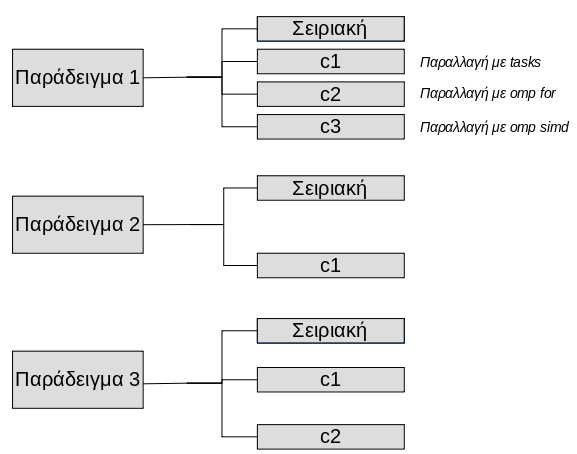
\includegraphics[width=0.5\textwidth]{diarthrosi_example}
\captionsetup{justification=centering, singlelinecheck=false}
\caption{Διάρθρωση παραδειγμάτων στο \href{https://github.com/gkonto/openmp/}{\emph{\en{github.com}}}}
\label{fig:diarthrosi_example}
\end{figure}
\end{center}

Για παράδειγμα, έστω ότι επιλύεται ένα πρόβλημα που ονομάζεται \emph{\en{Foo}} με διαφορετικές παραλλαγές μιας
συνάρτησης \emph{\en{fun()}}. Τότε δημιουργείται ένα κεντρικό αρχείο \emph{\en{run.cpp}} που περιέχει τη
\emph{\en{main()}} και σε κάθε υποφάκελο (\emph{\en{c1, c2}}) ένα αρχείο \emph{\en{test.cpp}} με διαφορετική παραλλαγή
της \emph{\en{fun()}}. Τότε στο αρχείο \en{run.cpp} γίνεται \emph{\en{\#include "test.hpp"}} και η εντολές για
\emph{\en{compile}} θα είναι οι εξής:\\
\en{g++ run.cpp ./c1/test.hpp -I c1}\\
\en{g++ run.cpp ./c2/test.hpp -I c2}
\clearpage
\subsection{Αρχιτεκτονική μηχανήματος και επιλογές μεταγλώττισης}
Τα προβλήματα που ακολουθούν εκτελέστηκαν σε μηχάνημα με λειτουργικό \emph{\en{linux}} και μεταγλωττιστή
\emph{\en{gcc-7.5.0}}. Οι προδιαγραφές υλικού του μηχανήματος που εκτελέστηκαν τα προβλήματα, αναφέρονται στον πίνακα που ακολουθεί. Για τη μεταγλώττιση των παραλλαγών χρησιμοποιήθηκε η επιλογή -Ο2, με σκοπό την εξαγωγή συμπερασμάτων σχετικά με τη διανυσματικοποίηση μέσω της οδηγίας \emph{\en{simd}} σύμφωνα με την οποία δεν υπάρχει υποκείμενη διανυσματικοποίηση. Ακόμη, γίνεται η χρήση της εντολής \en{no-inline} με σκοπό την απαγόρευση της μετατροπής συναρτήσεων σε \en{inline} αυτόματα από το μεταγλωττιστή, για την αποφυγή εσφαλμένων συμπερασμάτων σχετικά με τη βελτίωση της απόδοσης από άλλους παράγοντες. Αξίζει επίσης να σημειωθεί η χρήση της επιλογής \en{-fno-stack-protector} σε παραλλαγές με χρήση \en{GPU}. Η επιλογή απαιτείται σε προβλήματα δέσμευσης μεγάλου τμήματος \en{stack} μνήμης. Περισσότερες λεπτομέρειες σχετικά με τις επιλογές μεταγλώττισης δίνονται στις επιμέρους παραλλαγές.

\selectlanguage{greek}
\begin{center}
\begin{table}[htbp]
\centering
\captionsetup{justification=raggedright,
singlelinecheck=false
}
\caption{Χαρακτηριστικά Μηχανήματος Εκτέλεσης}
\def\arraystretch{1.5}
\begin{tabular}{| p{0.25\textwidth} | p{0.25\textwidth}|}
\hline
 \en{\textbf{Architecture}}  \cellcolor[HTML]{D0D0D0} & \en{x86\_64}  \\
\hline
 \en{\textbf{CPU op-mode(s)}} \cellcolor[HTML]{D0D0D0} & \en{32-bit, 64-bit} \\
\hline
 \en{\textbf{CPU(s)}} \cellcolor[HTML]{D0D0D0}  & 16\\
\hline
 \en{\textbf{Thread(s) per core}} \cellcolor[HTML]{D0D0D0} & 1 \\
\hline
 \en{\textbf{Core(s) per socket}} \cellcolor[HTML]{D0D0D0} & 8\\
\hline
 \en{\textbf{Socket(s)}} \cellcolor[HTML]{D0D0D0} & 2 \\
\hline
 \en{\textbf{NUMA node(s)}} \cellcolor[HTML]{D0D0D0} & 4\\
\hline
 \en{\textbf{Model name}} \cellcolor[HTML]{D0D0D0}  &  \en{AMD Opteron(tm) Processor 6128 HE}\\
\hline
\en{\textbf{L1d cache}} \cellcolor[HTML]{D0D0D0} &  \en{64K} \\
\hline
\en{\textbf{L2 cache}} \cellcolor[HTML]{D0D0D0} & \en{512K}  \\
\hline
\en{\textbf{L3 cache}} \cellcolor[HTML]{D0D0D0} & \en{5118K}  \\
\hline
 \en{\textbf{Memory}} \cellcolor[HTML]{D0D0D0} & 16036\\
\hline
\end{tabular}
\end{table}
\end{center}

 

\clearpage